\section{问题的形式化 (Formalizing the Problem)}

为了能够严谨地分析信息销售问题,我们首先需要建立一个统一的数学语言。

\subsection{核心要素:上下文 (Context) $(u,\mu)$}

整个信息销售问题可以被一个我们称为上下文(Context)的元组$(u, \mu)$所概括。这个上下文是买卖双方的共同知识(Common Knowledge)。

它包含以下核心要素:

\textbf{世界状态 (State of the World)}:$\omega \in \Omega$。这是一个随机变量,代表了客观世界中一个不确定的、但与决策收益相关的状态。$\Omega$是所有可能状态的有限集合。

\textbf{卖方私有信号 (Seller's Private Signal)}:在本模型的基本设定中,我们假设卖方完全知晓世界状态$\omega$。所以,$\omega$就是卖方的私有信息。

\textbf{买方私有类型 (Buyer's Private Type)}:$\theta \in \Theta$。这也是一个随机变量,代表了买方在交易开始前就拥有的私有信息。$\Theta$是所有可能类型的有限集合。$\theta$可以包含多种信息:
\begin{enumerate}
    \item 买方关于$\omega$的信号:$\theta$可能是$\omega$的一个不完美的、带有噪声的观测。
    \item 买方的偏好:$\theta$也可以代表买方自身的效用函数差异。
\end{enumerate}
我们统一用$\theta$来表示买方所有的私有信息。

\textbf{买方行动 (Buyer's Actions)}:$a\in A$。这是买方在获得信息后可以选择的决策集合,$A$是一个有限集。

\textbf{效用函数 (Utility Function)}:$u(\theta, \omega, a) \to \mathbb{R}$。这个函数描述了买方的收益。当买方的私有类型是$\theta$,世界真实状态是$\omega$,且买方采取了行动$a$时,他获得的收益是$u(\theta, \omega, a)$。这个函数是整个模型的核心,它将信息和行动的价值联系了起来。

\textbf{联合概率分布 (Joint Probability Distribution)}:$\mu(\omega, \theta)$。这是一个在$\Omega \times \Theta$上的联合概率分布,是所有参与者的共同知识。$\mu(\omega, \theta)= \Pr(\text{世界状态}=\omega, \text{买方类型}=\theta)$。

这个分布描述了卖方和买方私有信息之间的相关性。如果$\mu(\omega,\theta)=\mu(\omega)\mu(\theta)$,我们称卖方和买方信号独立。否则,称之为相关。例如,如果富有的买方(一种$\theta$)更有可能是跑车爱好者(一种$\omega$),那么$\omega$和$\theta$就是相关的。

\subsection{买方的目标:最大化效用}

一个理性的买方,其目标是在其所知信息的约束下,选择一个行动$a$来最大化自己的期望效用。

\textbf{无额外信息时的期望效用 (Status Quo Utility)}

在与卖方交易之前,类型为$\theta$的买方只知道自己的$\theta$。他需要基于$\theta$对$\omega$形成一个后验信念。根据贝叶斯法则,$\omega$的条件概率分布是$\Pr(\omega | \theta) = \mu(\omega,\theta)/\mu(\theta)$,其中$\mu(\theta)=\sum\limits_{\omega^\prime} \mu(\omega^\prime, \theta)$。

因此,他的最优决策是选择一个$a$来最大化期望效用:
$$U_{\text{prior}}(\theta) = \max_{a\in A}\mathbb{E}_{\omega\sim \mu(\cdot|\theta)}[u(\theta,\omega,a)]=\max_{a\in A}\sum\limits_{\omega\in\Omega}\frac{\mu(\omega,\theta)}{\mu(\theta)}u(\theta,\omega,a)$$

这是买方的保留效用(Reservation Utility)或外部选项(Outside Option),即他不参与交易所能获得的最低保证效用。

\textbf{拥有完全信息时的期望效用 (Full Information Utility)}

假设一个理想情况,卖方免费将信息$\omega$完整地告诉了买方。那么对于每一个可能的$\omega$,买方都可以选择最优的行动$a$。他此时的期望效用是:
$$U_{\text{post}}(\theta)=\mathbb{E}_{\omega\sim\mu(\cdot|\theta)}[\max_{a\in A} u(\theta,\omega,a)] = \sum\limits_{\omega\in\Omega}\frac{\mu(\omega,\theta)}{\mu(\theta)}\max_{a\in A}u(\theta,\omega,a)$$

\textbf{信息的价值 (Value of Information)}

对一个类型为$\theta$的买方而言,信息$\omega$的全部价值$\xi(\theta)$,就是拥有信息前后他能获得的最大期望效用之差:
$$\xi(\theta)=U_{\text{post}}(\theta)-U_{\text{prior}}(\theta) \geq 0$$

这个差值$\xi(\theta)$是非负的,因为拥有更多信息总不会让决策变得更差。$\xi(\theta)$代表了类型为$\theta$的买方愿意为获得完整信息$\omega$所支付的最高价格。如果价格超过$\xi(\theta)$,他宁愿不要这个信息,自己根据$\theta$去决策。

\subsection{卖方的目标:最大化收益}

卖方的目标是设计一个销售机制,从买方那里榨取尽可能多的价值。其总的期望收益(Revenue)是所有类型的买方支付的金额的期望值:

$$\text{Revenue} = \sum\limits_{\theta\in\Theta}\mu(\theta)\cdot t(\theta)$$

其中$t(\theta)$是卖方最终从类型为$\theta$的买方那里收取的期望费用。显然,卖方收取的费用不能超过信息的价值,即$t(\theta)\leq\xi(\theta)$。

卖方的挑战在于,她并不知道买方的真实类型$\theta$,所以她无法为每种类型"量身定做"一个价格$\xi(\theta)$。她必须设计一个对所有类型都有效的机制。
  
\subsection{初步尝试:"密封信封"机制 (The "Sealed Envelope" Mechanism)}

在深入复杂的机制之前,我们先分析一个最直观、最简单的方案,并看看它有什么问题。

\textbf{机制描述:}
\begin{enumerate}
    \item 卖方知道了真实的$\omega$。
    \item 她将$\omega$的值写在一张纸条上,放入一个信封。
    \item 她给这个信封定一个固定的、公开的价格$t$。
    \item 买方看到价格$t$后,自行决定是否购买。
\end{enumerate}

\textbf{买方的决策:}
一个类型为$\theta$的买方,其购买此信封的价值是$\xi(\theta)$。根据理性人假设,他会做出如下决策:
\begin{enumerate}
    \item 如果$\xi(\theta)\geq t$,他会购买。购买后,他的净效用是$\xi(\theta)-t$。
    \item 如果$\xi(\theta)<t$,他不会购买。他不购买的净效用是0。(为简化讨论,我们假设在$\xi(\theta)=t$时买方会购买。)
\end{enumerate}

\textbf{卖方的收益:}
卖方的期望收益是价格$t$乘以所有会购买的买方类型的概率之和:
$$\text{Revenue}(t) = t\cdot \sum\limits_{\theta: \xi(\theta)\geq t}\mu(\theta)$$

卖方的任务就变成了选择一个最优的价格$t^*$来最大化这个收益函数$\text{Revenue}(t)$。这本质上是一个经典的垄断定价问题。

\textbf{"密封信封"机制的缺陷:}
这个机制看起来简单,但它忽略了一个关键问题:卖方在得知$\omega$之后,可能会希望根据$\omega$的不同来调整价格$t$。

\textbf{一个失败的改进尝试:}
卖方可能会想:"对于不同的$\omega$,信息$\omega$对买方的价值可能是不同的。我为什么不根据$\omega$来定价呢?",即设置一个价格函数$t(\omega)$。

这恰恰是信息销售的微妙之处。一旦卖方这么做了,价格本身就携带了关于$\omega$的信息。

假设在广告例子中,$\omega=$"年轻单身"时信息价值高,卖方定价$t($年轻单身$)= 1000$元;$\omega=$"中年有孩"时信息价值低,卖方定价$t($中年有孩$) = 100$元。买方过来一询价,卖方报价"1000元"。此时,即使买方一分钱没付,他也立刻能推断出$\omega$极有可能是"年轻单身"。他已经免费获得了信息,为什么还要付费呢?

这个简单的例子揭示了设计信息销售机制的核心困难:任何与卖方私有信息$\omega$相关的机制元素(如价格、信息披露的颗粒度等),都可能成为泄露信息的渠道。买方可以利用这些渠道进行"投机",在不完全付费的情况下获取信息。

因此,我们需要一个更强大、更通用的框架来描述和分析所有可能的、包含复杂交互的销售协议。

\subsection{示例}

为了更具体地理解$\xi(\theta)$的计算和"密封信封"机制的收益,我们可以用Python写一个简单的模拟。

\textbf{场景设定:}
\begin{itemize}
    \item 世界状态$\Omega=\{0,1\}$
    \item 买方行动$A=\{0,1\}$
    \item 买方类型$\Theta=\{0,1\}$
    \item 联合分布$\mu(\omega,\theta)$:
       \begin{itemize}
          \item $\mu(\omega=0,\theta=0)=0.4$
          \item $\mu(\omega=1,\theta=0)=0.1$
          \item $\mu(\omega=0,\theta=1)=0.1$
          \item $\mu(\omega=1,\theta=1)=0.4$
          \item 这表明$\theta$是$\omega$的一个强信号,$\theta=0$暗示$\omega=0$,$\theta=1$暗示$\omega=1$。
       \end{itemize}
    \item 效用函数$u(\theta,\omega,a)$:假设效用只和$\omega$与$a$是否匹配有关,$\theta$只影响买方的先验信念。
       \begin{itemize}
          \item $u(\omega,a)=10$ 如果$\omega=a$(行动正确)
          \item $u(\omega,a)=0$ 如果$\omega\neq a$(行动错误)
       \end{itemize}
\end{itemize}

以下是实现的Python代码,完整的程序在同级目录下的program1.py程序。

\begin{lstlisting}[language=Python,style=pythonstyle]
    import numpy as np
    import matplotlib.pyplot as plt
    
    class Context:
        def __init__(self):
            self.Omega = [0, 1]
            self.Theta = [0, 1]
            self.A = [0, 1]
            
            self.mu_joint = np.array([[0.4, 0.1],  # theta=0: mu(omega=0|theta=0)=0.4, mu(omega=1|theta=0)=0.1
                                      [0.1, 0.4]]) # theta=1: mu(omega=0|theta=1)=0.1, mu(omega=1|theta=1)=0.4
            
            self.mu_theta = np.sum(self.mu_joint, axis=0) # [0.5, 0.5]
            self.mu_omega = np.sum(self.mu_joint, axis=1) # [0.5, 0.5]
            
            self.mu_cond_w_given_t = self.mu_joint / self.mu_theta
            
        def u(self, omega, action):
            return 10.0 if omega == action else 0.0
    
    def calculate_xi(context, theta):
        expected_utilities_prior = []
        for action in context.A:
            utility = 0
            for omega_idx, omega in enumerate(context.Omega):
                prob_w = context.mu_cond_w_given_t[omega_idx, theta]
                utility += prob_w * context.u(omega, action)
            expected_utilities_prior.append(utility)
        
        u_prior = np.max(expected_utilities_prior)
        best_action_prior = np.argmax(expected_utilities_prior)
    
        u_post = 0
        for omega_idx, omega in enumerate(context.Omega):
            prob_w = context.mu_cond_w_given_t[omega_idx, theta]

            best_utility_for_omega = 0
            for action in context.A:
                best_utility_for_omega = max(best_utility_for_omega, context.u(omega, action))
            
            u_post += prob_w * best_utility_for_omega
    
        xi = u_post - u_prior
        return xi
    
    def sealed_envelope_revenue(t, xi_values, mu_theta):

        revenue = 0
        for theta_idx, xi in enumerate(xi_values):
            if xi >= t:
                revenue += t * mu_theta[theta_idx]
        return revenue
    
    if __name__ == "__main__":
        ctx = Context()

        xi_values = [calculate_xi(ctx, theta) for theta in ctx.Theta]

        prices_to_test = np.linspace(0, max(xi_values) + 1, 1000)
        revenues = [sealed_envelope_revenue(t, xi_values, ctx.mu_theta) for t in prices_to_test]
        
        max_revenue = np.max(revenues)
        optimal_price = prices_to_test[np.argmax(revenues)]
    
        plt.figure(figsize=(10, 6))
        plt.plot(prices_to_test, revenues)
        plt.title("Revenue of Sealed Envelope Mechanism vs. Price (t)")
        plt.xlabel("Price (t)")
        plt.ylabel("Expected Revenue")
        plt.axvline(x=optimal_price, color='r', linestyle='--', label=f'Optimal Price t* = {optimal_price:.2f}')
        plt.grid(True)
        plt.legend()
        plt.show()    
\end{lstlisting}

\begin{figure}[H]
    \centering
    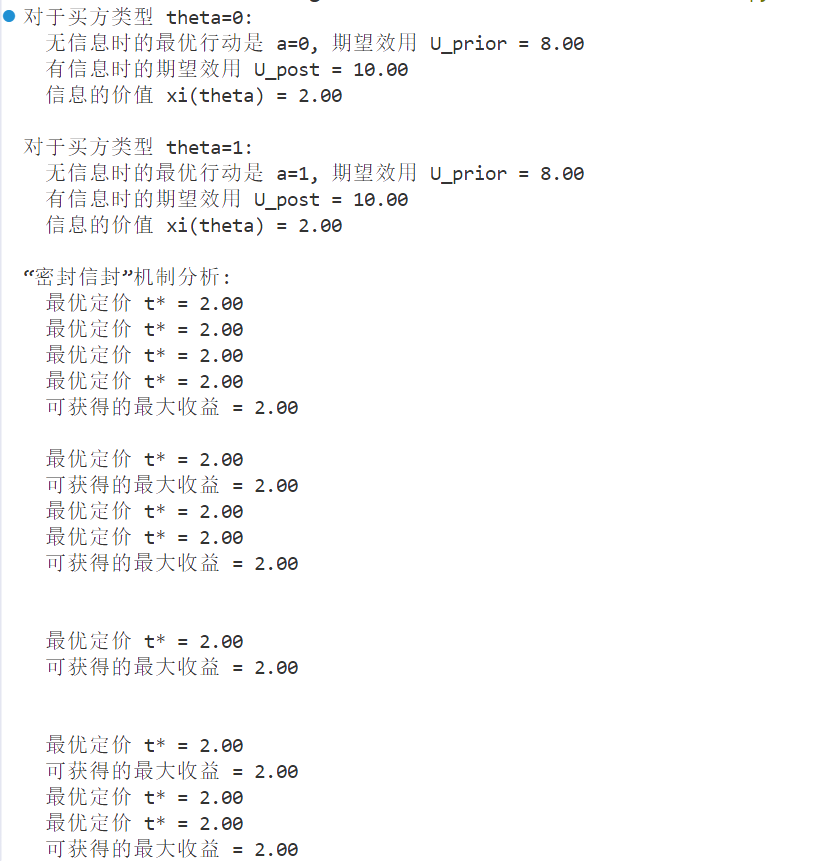
\includegraphics[width=0.6\linewidth]{image15.png}
    \caption{密封信封机制的收益优化结果}
    \label{fig:result}
\end{figure}

代码运行结果如下:
\begin{figure}[H]
    \centering
    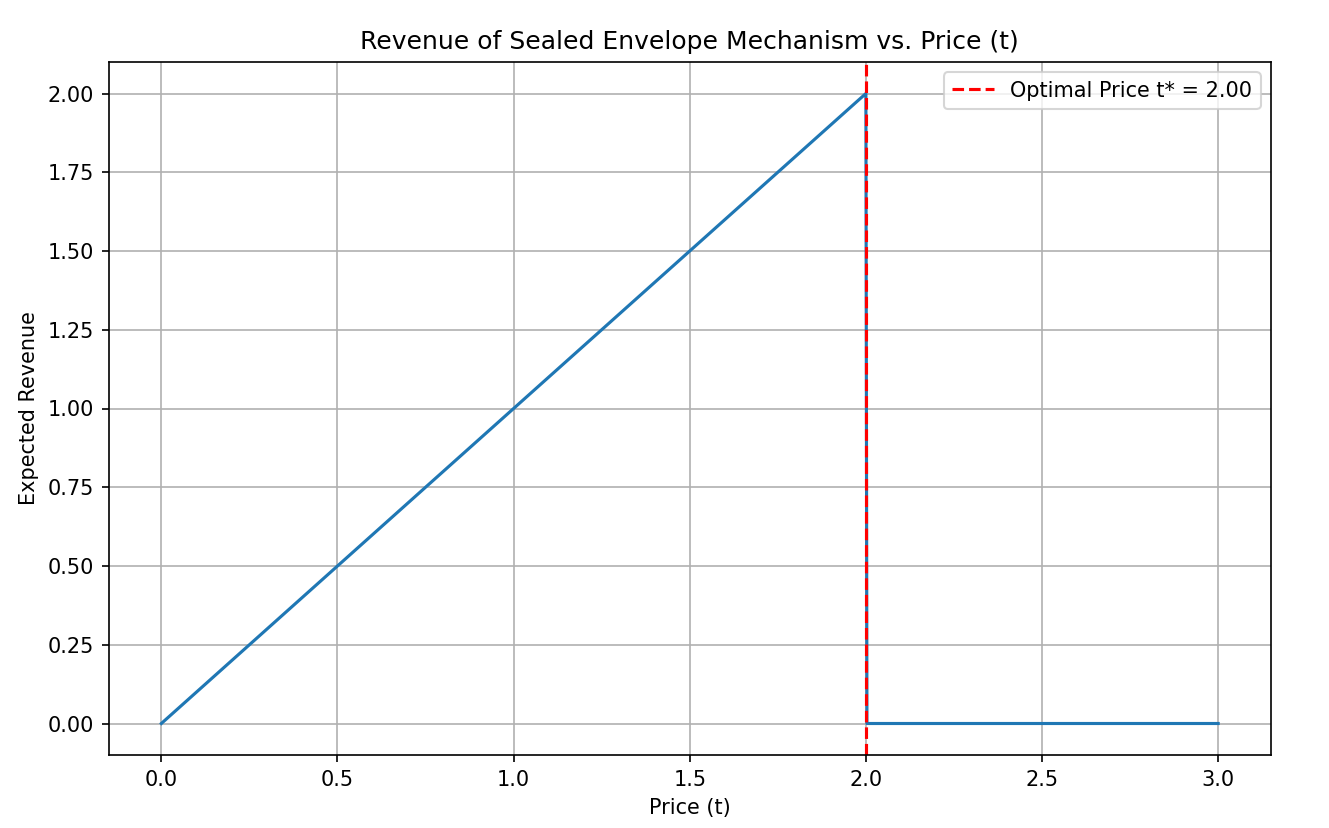
\includegraphics[width=0.5\linewidth]{image14.png}
    \caption{收益函数的可视化结果}
    \label{fig:visualization}
\end{figure}

在这个特定的例子中,两种类型的买方$\theta=0$和$\theta=1$恰好具有相同的信息价值$\xi(\theta)=2.0$。因此,卖方最优的定价就是$t^*=2.0$,此时两种类型的买方都会购买,卖方的总收益为:
$$t^* \times (\mu(\theta=0) + \mu(\theta=1)) = 2.0 \times (0.5 + 0.5) = 2.0$$

这个简单的代码示例,将前面定义的抽象概念(上下文、效用、信息价值)转化为了可计算的实体,并直观地展示了最简单的"密封信封"机制是如何运作和优化的。然而,正如我们所分析的,这个简单机制的背后隐藏着深刻的缺陷,这促使我们必须进入下一章,探索更一般、更强大的机制。